% Mixed block-causal attention mask — TikZ source. Compiles to a tight standalone
% PDF (pdflatex figures/mixed-mask.tex), which `book-scaffold build-figures`
% converts to public/figures/mixed-mask.svg.
%
% Causal (lower-triangular) across the stream, with a full bidirectional block
% inside an image segment (positions 3..5). All-text limit drops the block and
% recovers the plain causal mask.
\documentclass[tikz,border=3pt]{standalone}
\usepackage{amsmath}
\usepackage{amssymb}
\usepackage{tikz}
\begin{document}
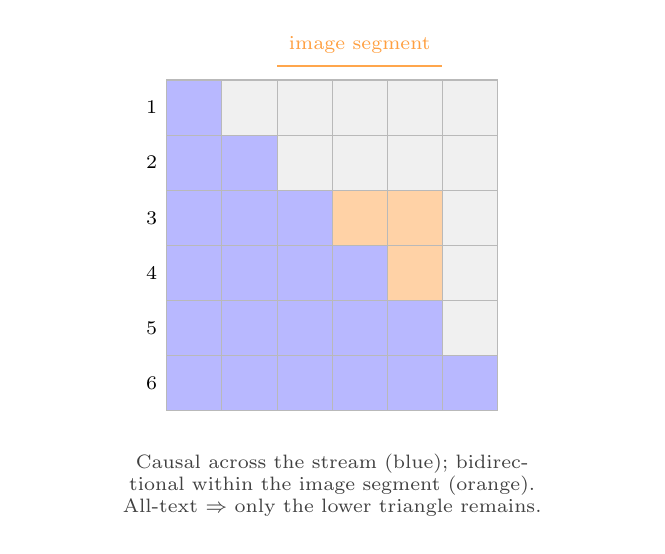
\begin{tikzpicture}[scale=0.7]
  % image segment = positions 3,4,5 (0-indexed 2,3,4)
  \foreach \i in {0,1,2,3,4,5} {
    \foreach \j in {0,1,2,3,4,5} {
      \pgfmathtruncatemacro{\causal}{\j<=\i ? 1 : 0}
      \pgfmathtruncatemacro{\imgblk}{ (\i>=2 && \i<=4 && \j>=2 && \j<=4) ? 1 : 0}
      \ifnum\causal=1
        \fill[blue!28] (\j,-\i) rectangle ++(1,-1);
      \else
        \ifnum\imgblk=1
          \fill[orange!35] (\j,-\i) rectangle ++(1,-1);
        \else
          \fill[black!6] (\j,-\i) rectangle ++(1,-1);
        \fi
      \fi
      \draw[gray!55] (\j,-\i) rectangle ++(1,-1);
    }
  }
  % image-segment bracket
  \draw[orange!70, thick] (2,0.25) -- (5,0.25);
  \node[above, font=\scriptsize, text=orange!75] at (3.5,0.3) {image segment};
  \foreach \i/\lbl in {0/{$1$},1/{$2$},2/{$3$},3/{$4$},4/{$5$},5/{$6$}}
    \node[left, font=\scriptsize] at (0,-\i-0.5) {\lbl};
  \node[below, align=center, text width=7.5cm, font=\scriptsize, text=black!75]
    at (3,-6.6)
    {Causal across the stream (blue); bidirectional within the image segment
     (orange). All-text $\Rightarrow$ only the lower triangle remains.};
\end{tikzpicture}
\end{document}
